%#BIBTEX bibtex Si$_3$N$_4$
\documentclass[twocolumn,amsmath,amssymb,a4paper,prb,superscriptaddress,floatfix]{revtex4-1}
\usepackage[dvipdfmx]{graphicx}
\usepackage{natbib}
\usepackage{multirow}
\usepackage{amsmath}
\usepackage{bm}
\usepackage{mathrsfs}
\usepackage{url}
\usepackage{color}
\usepackage{ulem}
\begin{document}

\title{First-principles calculation of the lattice thermal
conductivities of $\alpha$-, $\beta$-, and $\gamma$-Si$_3$N$_4$}

\author{Kazuyoshi Tatsumi} \email{k-tatsumi@imass.nagoya-u.ac.jp}
\affiliation{Advanced Measurement Technology Center, Institute of
Materials and Systems for Sustainability, Nagoya University, Chikusa,
Nagoya 464-8603, Japan}
\affiliation{Center for Elements Strategy
Initiative for Structural Materials, Kyoto University, Sakyo, Kyoto
606-8501, Japan}

\author{Atsushi Togo}
\affiliation{Center for Elements Strategy Initiative for Structural
Materials, Kyoto University, Sakyo, Kyoto 606-8501, Japan}

\author{Isao Tanaka}
\affiliation{Center for Elements Strategy Initiative for Structural
Materials, Kyoto University, Sakyo, Kyoto 606-8501, Japan}
\affiliation{Department of Materials Science and
Engineering, Kyoto University, Sakyo, Kyoto 606-8501, Japan}
\affiliation{Nanostructures Research Laboratory, Japan Fine Ceramics
Center, Atsuta, Nagoya 456-8587, Japan}

\begin{abstract}
Lattice thermal conductivities of $\alpha$-, $\beta$- and
$\gamma$-Si$_3$N$_4$ single crystals are investigated from {\it
ab-initio} anharmonic lattice dynamics, within the single-mode
relaxation-time approximation of the linearized phonon Boltzmann
transport equation. At 300 K, the lattice thermal conductivity of
$\alpha$-Si$_3$N$_4$ is calculated as $\kappa_{xx}=69$ and
$\kappa_{zz}=99$ (in units of Wm$^{-1}$K$^{-1}$). For
$\beta$-Si$_3$N$_4$, $\kappa_{xx}=73$ and $\kappa_{zz}=198$ are
obtained, that is consistent with the reported experimental values of 69
and 180, respectively. The difference of anisotropy between
$\alpha$-Si$_3$N$_4$ and $\beta$-Si$_3$N$_4$ is originated from their
characteristic difference in the phonon band structures, although their
crystal structures are similar in their local atomic coordinates. In
$\alpha$-Si$_3$N$_4$, acoustic-mode phonons below 6 THz are the main
heat carriers. In $\beta$-Si$_3$N$_4$, the phonon modes up to 12 THz
contribute to the lattice thermal conductivity.
%
In $\gamma$-Si$_3$N$_4$, $\kappa=81$ is obtained. The distribution of phonon
mode contributions to lattice thermal conductivity with respect to phonon
frequency is found to closely resemble $\kappa_{xx}$ of $\beta$-Si$_3$N$_4$
although the phonon lifetimes of $\gamma$-Si$_3$N$_4$ are twice shorter than
those of $\beta$-Si$_3$N$_4$.
\end{abstract}

\maketitle

\section{Introduction}
Several nitride insulators exhibiting high thermal conductivities are important
for heat sink materials used at elevated temperatures. Wurtzite-type w-AlN,
which has an Adamantine (diamond-like) crystal structure, was noted by Slack
{\it et al.}~\cite{slack} as a superior thermal conductor over 100 Wm$^{-1}$K$^{-1}$.
Si$_3$N$_4$ has been more recently recognized as one of the good thermally
conductive insulators. Remarkable advances in ceramic technologies related to
the densification of the sintered body and microstructural control have pushed
the thermal conductivities of polycrystalline of Si$_3$N$_4$ ceramics up to 177
Wm$^{-1}$K$^{-1}$.~\cite{zhou,hirao,watari,hirosaki} Since Si$_3$N$_4$ ceramics
also exhibit high mechanical strength at elevated temperatures, they are
regarded as ideal materials for use in various applications, such as engine components,
gas turbines, and heat sink substrates of power semiconductor devices.

At atmospheric pressure, Si$_3$N$_4$ exists in one of two phases, $\alpha$ and
$\beta$, both in the hexagonal lattice system, which are generally considered
to be low- and high-temperature phases,
respectively.~\cite{zhou,hirosaki,riley} Their crystal structures are commonly
formed by stacking of basal layers of SiN$_4$ tetrahedra.  The stacking manners
in $\alpha$ and $\beta$-Si$_3$N$_4$ are as ABCDABCD.. and ABAB.., respectively.
This difference is depicted in Fig.~\ref{fig:Fig1_cryst} from the principal
axis direction.  
The CD layers are related to AB by the $c$ glide operation,~\cite{hampshire} along which the unit cell periodicity of the $\alpha$ phase
is approximately two times longer than that of the $\beta$ phase, with lattice
constants of $c$ = 5.62 \AA~\cite{yashima} and 2.91 \AA~\cite{boulay}, respectively.
In addition to these phases, a cubic spinel phase ($\gamma$-Si$_3$N$_4$) can be
formed upon compression and in-situ heating.~\cite{zerr,zhang} The reported
transition pressures were scattered from 10 to 36 GPa depending on the
experimental conditions.~\cite{xu}  The produced $\gamma$ phase can be experimentally
quenched to atmospheric pressure and room temperature.
\begin{figure}[ht]
 \begin{center}
  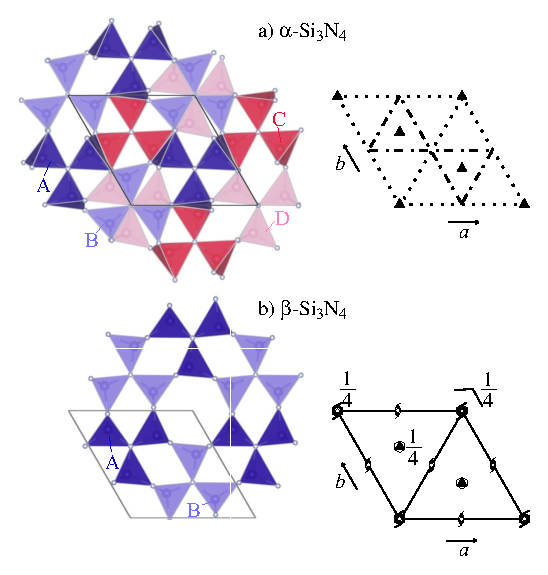
\includegraphics[width=0.90\linewidth]{Fig1_crystal_str2.eps} \caption{(color
  online) Crystal structures of $\alpha$- and $\beta$-Si$_3$N$_4$. Stacking of
  SiN$_4$ tetrahedron layers are shown in left. (a) ABCDABCD.. for
  $\alpha$-Si$_3$N$_4$. (b) ABAB.. for $\beta$-Si$_3$N$_4$.  Space group
  diagrams~\cite{inttableA} in P31c ($\alpha$-Si$_3$N$_4$) and P6$_3$/m ($\beta$-Si$_3$N$_4$)
  are shown in right.}
  \label{fig:Fig1_cryst} 
 \end{center}
\end{figure}

By using high-resolution thermoreflectance microscopy, Li {\it et
al.}~\cite{li} reported that the thermal conductivities of individual
rod-shaped $\beta$-Si$_3$N$_4$ grains in a ceramic were 69 and 180
Wm$^{-1}$K$^{-1}$ along the $a$ and $c$ axes, respectively, and thus suggested
its large anisotropy in thermal conductivity.  Takahashi {\it et al.}~\cite{takahashi} have recently developed a technique by which
$\beta$-Si$_3$N$_4$ grains are coated with graphene of relatively high magnetic
susceptibility, enabling them to align their $c$ axis along the external
magnetic field.  Based on this technique, it has been proposed that the
textural structure of rod-shaped $\beta$-Si$_3$N$_4$ grains would increase
their thermal conductivity to a level matching or exceeding that of w-AlN. 

Although the fabrication of millimeter-sized $\beta$-Si$_3$N$_4$ single
crystals has been reported,~\cite{yamamoto} the thermal conductivity of an
isolated single crystal of any Si$_3$N$_4$ phase has not yet been
experimentally determined.  It was proposed that the anisotropy in the thermal
conductivity of $\beta$-Si$_3$N$_4$ phase grains may not stem from the
intrinsic crystal properties, but rather, from the selective removal of crystal
defects along the $c$ axis of the grains.~\cite{watari-trans} Theoretically,
Hirosaki {\it et al.}~\cite{hirosaki-md} estimated the room-temperature lattice
thermal conductivities (LTCs) $\kappa$$_{xx}$ and $\kappa$$_{zz}$ of
$\alpha$-Si$_3$N$_4$ to be 105 and 225 Wm$^{-1}$K$^{-1}$, and those of
$\beta$-Si$_3$N$_4$ to be 170 and 450 Wm$^{-1}$K$^{-1}$, respectively, by
applying the Green-Kubo formulation to the molecular dynamics (MD) method with
the interatomic potentials proposed by Vashishta {\it et al.}~\cite{vashishta}
Although the absolute values were more tan two times larger, the ratio of the
LTCs in the $\beta$ phase along the $a$ and $c$ axes agreed well with the
experimental results obtained by Li {\it et al.}~\cite{li} Moreover, the MD
results suggest that the different stacking orders beween $\alpha$- and
$\beta$-Si$_3$N$_4$ alter their LTC largely. On the other hand, the recent LTC
calculation based on first principles calculation and Boltzman transport theory
has shown that in many polymorphs of the wurtzite and zincblende structures,
which have different stacking orders of the densest atom planes as ABAB.. and
ABCABC.., these orders merely alter the LTCs.~\cite{phono3py} It is interesting
to investigate it using this approach for $\alpha$- and $\beta$-Si$_3$N$_4$. 

In addition to these phases, a cubic spinel phase ($\gamma$-Si$_3$N$_4$) can be
formed upon compression and in-situ heating.~\cite{zerr,zhang} The reported
transition pressures were scattered from 10 to 36 GPa depending on the
experimental conditions.~\cite{xu}  The produced $\gamma$ phase can be experimentally
quenched to atmospheric pressure and room temperature.  Its thermal
conductivity has not been experimentally reported; it has been estimated only
by the Slack model.~\cite{morelli} 

The present study aims to qualitatively understand the LTC tensors among the
three Si$_3$N$_4$ phases by means of the first principles approach.  After the
methodology section, we examine the validity of the present LTC results first.
Then we investigate the characteristics in the LTCs in detail.

\section{Computational procedures}

\subsection{Lattice thermal conductivity calculation}

The LTCs were calculated by solving the linearized Boltzmann transport equation
(LBTE) within the single-mode relaxation time approximation (single-mode RTA).
We also tried the direct-solution of LBTE~\cite{chaput-direct} and
leave its calculated LTC values in the following section. The
difference of LTCs between by the single-mode RTA and by the direct solution
was found minor for our discussion. Therefore we limited our research to use
the single-mode RTA to take advantage of its intuitive closed form of LTCs.

In the following sections, we denote a phonon mode by $\lambda=(\mathbf{q},p)$
with the set of the phonon wave vector $\mathbf{q}$ and band index $p$ and $-\lambda \equiv (-\mathbf{q},p)$. The
relaxation time due to phonon-phonon scattering was obtained as reciprocal of
linewidth, $\tau_{\lambda,\text{ph-ph}}=(2\Gamma_\lambda)^{-1}$, where the
linewidth that we employed in this study is as follows:
\begin{align}
 \label{eq:linewidth}
 &\Gamma_\lambda = \frac{18\pi}{\hbar^2}
  \sum_{\lambda' \lambda''}
  \bigl|\Phi_{-\lambda\lambda'\lambda''}\bigl|^2 \times \nonumber \\ 
 &\left\{ (n_{\lambda'} + n_{\lambda''}+1) 
   \delta(\omega_\lambda-\omega_{\lambda'}-\omega_{\lambda''}) \right.
   + \nonumber \\ 
 &\;\;(n_{\lambda'}-n_{\lambda''})
  \left[\delta(\omega_\lambda +\omega_{\lambda'}-\omega_{\lambda''})
 \right. 
 \left. -\left. \delta(\omega_\lambda - \omega_{\lambda'}+\omega_{\lambda''})
 \right]\right\}.
\end{align}
Here $\omega_\lambda$ is the harmonic phonon frequency of the phonon mode
$\lambda$, $n_\lambda=[\exp(\hbar\omega_\lambda/\mathrm{k_B}T)-1]^{-1}$ is
the Bose-Einstein distribution at temperature $T$, and
$\Phi_{\lambda\lambda'\lambda''}$ denotes the three-phonon-scattering strength.
$\Phi_{\lambda\lambda'\lambda''}$ was obtained by usual coordinate
transformation of third-order IFCs from direct space to phonon
space.~\cite{phono3py} The second- and third-order real-space IFCs
were obtained from the {\it ab-initio} calculation, whose details are written in the
next section.

In order to compare the more realistic results of the calculated LTC with the
experimental data, the isotopic scattering effect due to the natural isotope
distribution was taken into account according to the second-order perturbation
theory.~\cite{tamura} With the relaxation times of the phonon-phonon scattering
and isotopic scattering, $\tau_{\lambda,\text{ph-ph}}$ and
$\tau_{\lambda,\text{iso}}$, the total relaxation time for a phonon mode was
assumed to be $1/\tau_{\lambda} = 1/\tau_{\lambda,\text{ph-ph}} +
1/\tau_{\lambda,\text{iso}}$, according to Matthiessen's rule.

These LTCs were calculated with the phonon-phonon interaction calculation code
PHONO3PY,~\cite{phono3py} while the harmonic phonon states were analyzed with
the phonon calculation code PHONOPY.~\cite{phonopy} 

The available experimental thermal conductivity data of the Si$_3$N$_4$ system
have been measured on the polycrystalline samples and not measured from any
single crystals. In order to consider the effect of various lattice defects in
the polycrystalline samples, such as grain boundaries, impurities, and
vacancies, we crudely took them into account by a relaxation time
$\tau_{\lambda,\text{bs}}=L/|\mathbf{v}_\lambda|$ of a phonon boundary
scattering model, where $\mathbf{v}_\lambda =
\nabla_{\mathbf{q}}\omega_\lambda$ is the group velocity and $L$ a
parameter regarding to the boundary mean free path. We consider
$\tau_{\lambda,\text{bs}}$ as a variable parameter and included it to
LTCs according to Matthiessen's rule.

The closed form of the LTC tensors within RTA were obtained via
\begin{align}
 \label{eq:kappa}
 \boldsymbol{\kappa}(T) = \frac{1}{N_\mathbf{q}\Omega} \sum_\lambda
 \tau_\lambda(T) \mathbf{v}_\lambda \otimes \mathbf{v}_\lambda c_\lambda(T),
\end{align}
where $N_\mathbf{q}$ is the number of
$\mathbf{q}$-points, $\Omega$ is the unit cell volume, and $c_\lambda$
is the mode heat capacity. To analyze the LTC in detail, we calculate
the cumulative thermal conductivity:
\begin{align}
 \label{eq:cum-kappa}
 \boldsymbol{\kappa}^\text{c}(\omega) = \frac{1}{N_\mathbf{q}\Omega}
 \int_0^\omega \sum_\lambda
 \tau_\lambda(T) \mathbf{v}_\lambda \otimes \mathbf{v}_\lambda
 c_\lambda(T) \delta(\omega'-\omega)d\omega',
\end{align}
and its derivative $\frac{\partial
\boldsymbol{\kappa}^\text{c}(\omega)}{\partial \omega}$ to see the phonon mode
contributions to the LTC.


\subsection{Computational details}

The IFCs were calculated using the first-principles projector
augmented wave method~\cite{paw} (VASP code~\cite{vasp-1996,vasp-1995,
vasp-1999}). The generalized gradient approximation (GGA) parameterized by
Perdew, Burke, and Ernzerhof~\cite{pbe} was used for the exchange correlation
potential. A plane wave energy cutoff of 500 eV was employed. The crystal
structures were optimized until the convergence in the residual forces acting
on the constituent atoms was less than $10^{-6}$ eV/\AA. The structural
optimization was firstly performed for a temperature of 0 K and 0 GPa. Here the
temperature and pressure were considered only for the electronic system and the
zero point lattice vibration was not taken into account. The calculated lattice
parameters were $a=7.808$ \AA~ and $c=5.659$ \AA~ for the $\alpha$ phase,
$a=7.660$ \AA~ and $c=2.925$ \AA~ for the $\beta$ phase, and $a=7.787$ \AA~
for the $\gamma$ phase, which agree with the experimental
data~\cite{yashima,boulay,paszkowicz} within +0.7 \% errors. The lattice
volume optimized at 0 K and 0 GPa within the local density approximation
(LDA)~\cite{lda} for the exchange correlation potential was, for
$\beta$-Si$_3$N$_4$, 3 \% smaller than the volume with GGA, which is a typical
volume contraction of LDA. In our test using $\beta$-Si$_3$N$_4$ at 0 K and 0
GPa, the LTC calculated with LDA was larger by 2.6 \% than that with GGA. For
our discussion, this difference is enough small, therefore the impact of
choice of exchange correlation potential is considered to be minor in our
study.

\begin{table}[ht]
	\caption{\label{table:LTC} Calculated lattice thermal conductivities 
 (LTC) of $\alpha$-, $\beta$-, and $\gamma$-Si$_3$N$_4$
 (WK$^{-1}$m$^{-1}$) at 300 K with respect to several combinations of
 supercell sizes.}
 \begin{ruledtabular}
  \begin{tabular}{ccccc}
   \multirow{2}{*}{Phase}
   & \multicolumn{2}{c}{Supercell (\# of atoms)} &
   \multicolumn{2}{c}{LTC} \\
   \cline{2-5}
   & $3^\text{rd}$ FC & $2^\text{nd}$ FC & $xx$ & $zz$ \\
   \hline
   \multirow{6}{*}{$\alpha$}
   & $1\times 1\times 1$ (28) & $1\times
   1\times 1$ (28) & \textcolor{blue}{37} &   \textcolor{blue}{57} \\ 
   & $1\times 1\times 2$ (56) & $1\times
   1\times 2$ (56) & \textcolor{blue}{41} &   \textcolor{blue}{79} \\ 
   & $1\times 1\times 1$ (28) & $2\times
   2\times 2$ (224) & \textcolor{blue}{55} &   \textcolor{blue}{81} \\ 
   & $1\times 1\times 2$ (56) & $2\times
   2\times 2$ (224) & \textcolor{blue}{67} &   \textcolor{blue}{95} \\ 
   & $1\times 1\times 2$ (56) & $2\times
   2\times 3$ (336) & \textcolor{blue}{68} &  \textcolor{blue}{97} \\ 
   & $1\times 1\times 2$ (56) & $3\times
   3\times 4$ (1008) & \textcolor{blue}{68} &  \textcolor{blue}{100} \\ 
   \hline
   \multirow{5}{*}{$\beta$}
   & $1\times 1\times 2$ (28) & $1\times
   1\times 2$ (28) & \textcolor{blue}{44} & \textcolor{blue}{173} \\ 
   & $1\times 1\times 2$ (28) & $2\times
   2\times 4$ (224) & \textcolor{blue}{76} &  \textcolor{blue}{208} \\ 
   & $1\times 1\times 3$ (42) & $2\times
   2\times 4$ (224) & \textcolor{blue}{71} & \textcolor{blue}{194} \\ 
   & $1\times 1\times 3$ (42) & $2\times
   2\times 5$ (280) & \textcolor{blue}{72} & \textcolor{blue}{196} \\ 
   & $1\times 1\times 3$ (42) & $3\times
   3\times 8$ (1008) & \textcolor{blue}{73} & \textcolor{blue}{199} \\ 
   \hline
   \multirow{3}{*}{$\gamma$}
   & $1\times 1\times 1$ (56) & $1\times
   1\times 1$ (56) & \multicolumn{2}{c}{\textcolor{blue}{72}} \\ 
   & $1\times 1\times 1$ (56) & $2\times
   2\times 2$ (448) & \multicolumn{2}{c}{\textcolor{blue}{77}} \\ 
   & $1\times 1\times 1$ (56) & $3\times
   3\times 3$ (56) & \multicolumn{2}{c}{\textcolor{blue}{79}} \\ 
  \end{tabular}
 \end{ruledtabular}
\end{table}

Supercell and finite difference approaches were used to calculate the
IFCs.~\cite{wei-supercell} The $1\times 1\times2$, $1\times 1\times3$, and
$1\times 1\times1$ supercells of the conventional unit cells were adopted for
the third-order IFCs of the $\alpha$, $\beta$, and $\gamma$ phases,
respectively, while the larger supercells $3\times 3\times4$, $3\times
3\times8$ and $2\times 2\times2$ were adopted for the respective second-order
IFCs.  The constant atomic displacement distance was set to 0.03 \AA.  Table
\ref{table:LTC} shows the calculated LTC values for several different choices
of supercell sizes, indicating that our calculated LTCs are reasonably
converging with respect to the supercell sizes. 

\textcolor{blue}{Non-analytical term correction~\cite{wang} was applied to the
second-order IFC to take into account the long range Coulomb forces present in
ionic crystals. For the correction, Born effective charges were calculated by
using the density functional perturbation theory (DFPT).}

Uniform $\mathbf{k}$-point sampling meshes of $4\times 4\times 2$,
$4\times 4\times 3$, and $3\times 3\times 3$ were used for the
third-order IFCs of the $\alpha$, $\beta$, and $\gamma$ phases. For the
former two phases the center of the $a^*$-$b^*$ plane were sampled
though the off-center grids along $c^*$-axis were sampled. For the
$\gamma$ phase, non-$\Gamma$ center mesh was used. For the second-order
IFC, the $\Gamma$-point was only sampled for the $\alpha$ and $\beta$
phase supercells and the only one $\mathbf{k}=(0.5, 0.5, 0.5)$ point was
sampled for the $\gamma$ phase supercell. The $\mathbf{q}$-point
sampling meshes of $10\times 10\times 14$, $10\times 10\times 26$, and
$12\times 12\times 12$ were used to calculate the LTCs in Eq.~(\ref{eq:kappa})
for the $\alpha$, $\beta$, and $\gamma$ phases.

To compare the calculated LTC with the experimental data measured at finite
temperatures, the experimentally measured lattice parameters may be preferred
in case that they are known. \textcolor{blue}{We examined LTC of $\beta$-Si$_3$N$_4$ at the
equilibrium volumes at 300, 600, 900, 1200 and 1500 K within the quasi-harmonic
approximation (QHA).~\cite{dove-p76} The LTC values with the equilibrium
lattice volumes within QHA were found to be deviated by less than 1 \% due to
the thermal expansions. The degree of the differences due to the thermal
expansions is similar to the case of Si and Ge~\cite{ward-ltc}. For the present
study, this effect is negligible and the LTC values calculated with the
equilibrium volume at 0 K are hereafter shown.}


We calculated volumetric thermal expansion coefficients and compared them with
the reported experimental values so as to check the validity of the present
calculation, because the thermal expansion is originated from the anharmonicity
of the interatomic potential as well as lattice thermal conduction. The
calculated values are 4.31$\times 10^{-6}$ and 4.19$\times 10^{-6}$ K$^{-1}$ at
300 K for the $\alpha$ and $\beta$ phases, while the experimental values were
3.75 and 3.55 ($10^{-6}$ K$^{-1}$)~\cite{minikayev-alpha}. The present
calculation reproduced the experimental tendency where the $\alpha$ phase has a
slightly larger thermal expansion coefficient than the $\beta$ phase,
supporting that the present calculations enable us to qualitatively compare the
LTC values of the Si$_3$N$_4$ phases.

In order to compare the microscopic phonon properties among the three phases at
the same conditions, those results calculated at 0 GPa are shown and discussed.
For the $\gamma$ phase, this means that we assume the condition of virtually
quenched $\gamma$ phase at 0 GPa from the high pressure. To examine the
analytical continuity of the properties with respect to pressures, we
calculated LTC of $\gamma$ phase at 10, 20, and 40 GPa as shown in
Fig.~\ref{fig:S1}, where the phenomenological behaviour of linear dependence of
LTC with respect to pressure with the calculated slope of 2.89
Wm$^{-1}$K$^{-1}$GPa$^{-1}$ was reproduced as similar to
Ref.~\onlinecite{andersson-pressure}. By this, we consider that the microscopic
values are also varied smoothly with the pressure and those at 0 GPa are
valuable to compare with the $\alpha$ and $\beta$ phases.

\subsection{Direct solution of LBTE}

The merit to employ the single-mode RTA for thermal conductivity calculation is
the closed form, by which we can intuitively understand the qualitative
character of LTC in terms of the relaxation time and group velocity. The
microscopic understanding of the full solution of LBTE is still under the
development~\cite{cepellotti-relaxons} and the microscopic picture based on
collective phonons~\cite{hardy-collective} will require more complicated
investigation although it is known that the single-mode RTA solution of LBTE
often underestimates the full solution.~\cite{mukhopadhyay-ltc,ward-ltc}

For the $\alpha$ and $\beta$ phases, we adopted a direct solution of
LBTE~\cite{chaput-direct}, which is one of the methods of LBTE full solutions.
The LTC values of the direct solution without the isotope effect were  69 and
102 Wm$^{-1}$K$^{-1}$ for $\kappa_{xx}$ and $\kappa_{zz}$  of the $\alpha$ phase
and 76 and 238 Wm$^{-1}$K$^{-1}$ for those of the $\beta$ phase, respectively, while the
corresponding single-mode RTA values were 70 and 102 Wm$^{-1}$K$^{-1}$ for the
$\alpha$ phase and 76 and 210 Wm$^{-1}$K$^{-1}$ for the $\beta$ phase. The
$\kappa_{zz}$ of the direct solution in the $\beta$ phase was 13 \% larger than
that of the single-mode RTA solution. Since the LTC difference between the LBTE
solutions is not significant, we expect the physics on LTC is well
understood within RTA in the current level of our interest.

\section{Results and discussion}

\subsection{Lattice thermal conductivities}

\begin{table}[ht]
 \caption{\label{table:LTC-exp} Calculated thermal conductivities of
 $\alpha$-Si$_3$N$_4$ (trigonal), $\beta$-Si$_3$N$_4$ (trigonal), and
 $\gamma$-Si$_3$N$_4$ (cubic) at 300
 K, compared with the experimental data. Theoretical bulk moduli $B$ in
 units of GPa, calculated by the authors by using the present band
 method, are presented in the fourth column.}
 \begin{ruledtabular}
  \begin{tabular}{cccccccccc}
   & \multicolumn{3}{c}{This work} & \multicolumn{3}{c}{\textcolor{red}{Ref. Theo.}}
   & \multicolumn{3}{c}{Ref. Expt.} \\
   \cline{2-10}
   & $\kappa_{xx}$ & $\kappa_{zz}$ & $B$ & $\kappa$ & $\kappa_{xx}$ & $\kappa_{zz}$ & $\kappa$ & $\kappa_{xx}$ & $\kappa_{zz}$ \\
   \hline
   $\alpha$-Si$_3$N$_4$ & \textcolor{blue}{68} & \textcolor{blue}{100} & 224 & 70\footnotemark[1] & 105\footnotemark[2] & 225\footnotemark[2] & 59\footnotemark[4] & - & -  \\
   $\beta$-Si$_3$N$_4$ & \textcolor{blue}{73} & \textcolor{blue}{199} & 237 & 250\footnotemark[1] & 170\footnotemark[2] & 450\footnotemark[2] & 122\footnotemark[5] & 69\footnotemark[6] & 180\footnotemark[6] \\
   $\gamma$-Si$_3$N$_4$ & \textcolor{blue}{77} & - & 296 & 80\footnotemark[1] & - & - & - & - & - 
   \footnotetext[1]{Ref.~\onlinecite{morelli}, Slack model.}
   \footnotetext[2]{Ref.~\onlinecite{hirosaki-md}, molecular dynamics (Green-Kubo).}
   \footnotetext[4]{Ref.~\onlinecite{hirai}, thin film.}
   \footnotetext[5]{Ref.~\onlinecite{hirosaki}, poly-crystals.}
   \footnotetext[6]{Ref.~\onlinecite{li}, single crystalline grains of poly-crystals.}
  \end{tabular}
 \end{ruledtabular}
\end{table}

In Table \ref{table:LTC-exp}, the theoretical LTCs at 300 K are compared with
the previously reported experimental~\cite{hirosaki,hirai,li} and
theoretical~\cite{morelli,hirosaki-md,phono3py} values. The present calculation
results better agree with the experimental $\kappa_{xx}$ and $\kappa_{zz}$ of
$\beta$-Si$_3$N$_4$, compared with the references of the Slack
model~\cite{morelli} and MD~\cite{hirosaki-md} results. The directional
averages of the present $\kappa_{ii}$ in the $\alpha$, $\beta$, and $\gamma$
phases are 79, 115, and 81 Wm$^{-1}$K$^{-1}$. The value of the $\gamma$ phase
is just as small as that of the $\alpha$ phase, although the former phase shows
the largest bulk modulus ($B$) in Table \ref{table:LTC-exp}.  It is generally
known that simple models through Debye temperature can provide only their rough
estimations.

It can be seen that the theoretical LTCs of $\beta$-Si$_3$N$_4$ are markedly
more anisotropic than those of the $\alpha$ phase. The theoretical LTCs of
$\beta$-Si$_3$N$_4$ are in good agreement with the corresponding experimental
data for individual grains reported by Li {\it et al.}~\cite{li}, indicating
that the experimentally reported large anisotropy in the thermal conductivities
of $\beta$-Si$_3$N$_4$ stems from the intrinsic properties of the crystal,
rather than specific defects induced during the sample preparation process.

Fig.~\ref{fig:Fig1_338} shows the theoretical LTCs of the $\alpha$  and $\beta$
phases as a function of $T$, in comparison with the reference experimental
data~\cite{hirosaki,hirai,li}, which were measured from the polycrystalline samples. The data of the
polycrystalline bulk samples cannot be directly compared with the theoretical
LTC tensors because the microstructures of the bulk samples affect the thermal
conductivities.  We calculate theoretical LTC values of the polycrystalline
bulk sample as $\kappa = w\kappa_{xx} + (1-w) \kappa_{zz}$, with an adjustable
parameter $w$ between 0 and 1 for the least square differences from the
experimental data.

\begin{figure}[ht]
 \begin{center}
  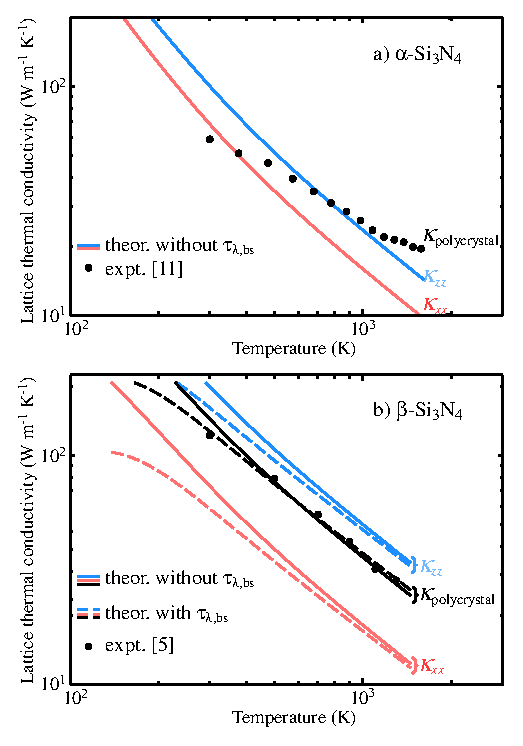
\includegraphics[width=0.90\linewidth]{Fig1_m1010.eps} \caption{(color
  online) Temperature dependence of LTC for $\alpha$-
  and $\beta$-Si$_3$N$_4$. For $\beta$-Si$_3$N$_4$, the LTC with the boundary scattering effect are
  shown by broken curves. Theoretical LTC for
  the bulk $\beta$-Si$_3$N$_4$ sample are also shown to be compared with
  the experimental data of the bulk sample.}
  \label{fig:Fig1_338}
 \end{center}
\end{figure}

The temperature dependence of the theoretical LTC, induced by
$\tau_{\lambda\text{,ph-ph}}$, is close to $T^{-1}$ because 300 K is high
enough to approximate the linewidth in Eq.~(\ref{eq:linewidth}) by a
high-temperature limit for these phases.  In Fig.~\ref{fig:Fig1_338}-a, the
temperature dependence of the experimental data of a chemically vapor-deposited
$\alpha$-Si$_3$N$_4$ sample~\cite{hirai} is deviated from $T^{-1}$
considerably, intersecting the theoretical curves of the $\kappa$$_{xx}$ and
$\kappa$$_{zz}$.  Thus no value of $w$ adjusts the theoretical LTC to the
experimental curve.  The full solution of LBTE would negligibly cure the
disagreement.  Including the simple phonon lifetime of boundary scattering,
$\tau_{\lambda,\text{bs}}=L/|\mathbf{v}_\lambda|$, into the total phonon
lifetime according to Matthiessen's rule, could not explain the discrepancy as
well.  $\tau_{\lambda,\text{bs}}=L/|\mathbf{v}_\lambda|$ with $L$ = \textcolor{blue}{0.6}
$\mu\text{m}$, which was much smaller than the experimental grain size 10
$\mu\text{m}$, decreases the room-temperature theoretical $\kappa$$_{xx}$ and
$\kappa$$_{zz}$ values toward the experimental values, but severely
underestimated the experimental values at the high temperature side.  At
present, the reason for the discrepancy between the theoretical and
experimental behaviors is unclear.  Although the crystal structure of the
experimental sample was characterized as $\alpha$-Si$_3$N$_4$, significant
lattice defects might exist in the as-deposited sample as pointed out by
Hirosaki {\it et al.}~\cite{hirosaki-md} and \textcolor{blue}{the simple phonon boundary
scattering model might fail to describe their effects.} The
experimental values of the $\beta$ phase ceramic bulk~\cite{hirosaki} in
Fig.~\ref{fig:Fig1_338}-b fall well between the calculated values of
$\kappa$$_{xx}$ and  $\kappa$$_{zz}$, being nearly parallel to the theoretical
$\kappa$$_{xx}$ and  $\kappa$$_{zz}$ curves.  If we compare the experimental
values with $\sum_i \kappa_{ii}/3$, which is a simple directional average, the
calculation shows slight underestimations with respect to the experiment, which
can be understood from an experimentally tailored microstructure containing
large $\beta$-Si$_3$N$_4$ grains selectively grown along the $c$
axis.~\cite{hirosaki}

The theoretical curve adjusted with $w=\textcolor{blue}{0.44}$ explains well the experimental
data of the poly-crystal bulk in Fig.~\ref{fig:Fig1_338}-b.  For the effects of
lattice defects most of which are grain boundaries, we included
$\tau_{\lambda,\text{BS}}$ with $L = \textcolor{blue}{0.6}$ $\mu\text{m}$ to further fit the
theoretical curve ($w=\textcolor{blue}{0.33}$) to the experimental data.  The $L$ value is
\textcolor{blue}{slightly smaller than} the average grain size (2 $\mu\text{m}$)~\cite{hirosaki} of the
experimental polycrystalline sample.  Fig.~\ref{fig:Fig1_338}-b also contains
the experimental $\kappa$$_{xx}$ and $\kappa$$_{zz}$ at room temperature by
filled squares, which are in-between the theoretical components with and
without $\tau_{\lambda,\text{BS}}$. 

\subsection{Dispersion curves}

Figure \ref{fig:Fig4_ver5_338} shows the phonon band diagrams of the three
Si$_3$N$_4$ phases. The entire band diagrams are almost identical to those
reported earlier~\cite{kuwabara,xu}. However, here we focus on the group
velocities on high-symmetry paths for the entire frequency range. This has not
been investigated by the previous works.

\begin{figure}[ht]
 \begin{center}
  \includegraphics[width=0.90\linewidth]{Fig4_ver5_338_resize2_woDOS.eps}
  \caption{(color online) Brillouin-zones (left) and calculated phonon band diagrams (right) for three Si$_3$N$_4$ phases.
  \label{fig:Fig4_ver5_338} }
 \end{center}
\end{figure}

The acoustic branches in the $\alpha$ phase highlighted in red in
Fig.~\ref{fig:Fig4_ver5_338}-a do not increase their frequencies much more than
those along the other paths, $\Gamma$--K or $\Gamma$--M. The frequency maxima
along the $\Gamma$--A path are around 7 THz, rather close to the maxima along
the $\Gamma$--K and $\Gamma$--M paths (around 5 THz). The upper branches along
the $\Gamma$--A path are also as flat as the upper branches along the
$\Gamma$--K and $\Gamma$--M paths.  In contrast, in the band diagram of the
$\beta$ phase (Fig.~\ref{fig:Fig4_ver5_338}-b), the acoustic phonon branches
highlighted in red along the $\Gamma$--A path increase their frequencies almost
linearly from the $\Gamma$-point to the A-point and reach around 10 THz, along
which the group velocity component $v_{\lambda,z}$ maintains high values. This
difference is because the $\Gamma$--A path length of the $\beta$ phase is
approximately twice that of $\alpha$; the lattice constant $c$ of $\beta$ is
nearly half that of $\alpha$, owing to the difference in the stacking manner of
the basal layers. Normally, optical branches are flat; however, the upper
branches along the $\Gamma$--A path also have significantly large
${v}_{\lambda,z}$.  In Fig.~\ref{fig:Fig4_ver5_338}-c for the $\gamma$
phase, the acoustic phonon branches highlighted in red show significant linear
dispersions. The frequencies of the longitudinal acoustic modes are 14 and 12.5
THz at the L-- and X--points. The frequencies of the transverse acoustic modes
are approximately half the values of the longitudinal modes at the L--point and
a factor of $1/\sqrt{2}$ smaller than the longitudinal modes at the X-point, as
in the case of fcc rare gas solids~\cite{dove-p30}. The roughly constant
gradients of the branches are large, reflecting the large elastic constants of
the $\gamma$ phase as shown in Table \ref{table:LTC-exp}.

\subsection{$\omega_\lambda$ counter map on reciprocal plane}

\begin{figure}[ht]
 \centerins
  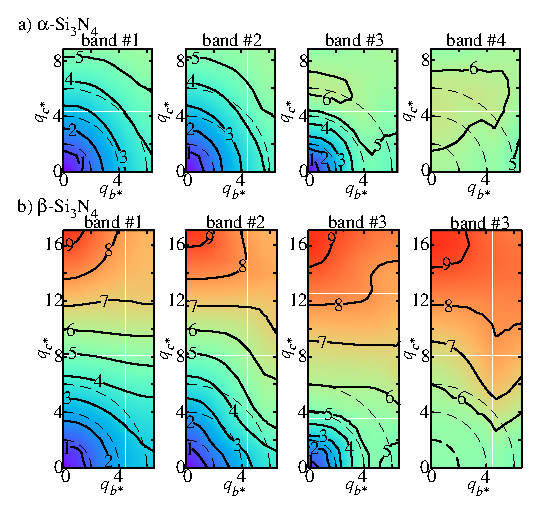
\includegraphics[width=\linewidth]{Fig2_small.eps} \caption{(color
  online) Contour maps of phonon frequency (THz) on the $b^*$-$c^*$
  planes of Brillouin-zones. The maps for the four lowest-frequency
  phonon states are shown. The frequency landscapes are formed by simply
  connecting the frequencies of the same band indices, assigned by
  ascending order of frequency at the respective $\mathbf {q}$
  points. \label{fig:Fig3_338} }
 \centering
\end{figure}

In another point of view on the group velocities, Fig.~\ref{fig:Fig3_338} shows
the cross-sections of the phonon frequency distributions on the $b^*$-$c^*$
planes in the first Brillouin-zones.  The cross-sections of other planes
containing the $c^*$ axis did not differ much from Fig.~\ref{fig:Fig3_338};
thus, we focus on the results for the $b^*$-$c^*$ planes as representative of
all such planes. We show only the frequencies of four modes from the lowest
frequency because they contribute significantly to LTC.
Fig.~\ref{fig:Fig3_338}-a shows that the frequency distributions and group
velocities of $\alpha$-Si$_3$N$_4$ are fairly isotropic.  On the other hand, in
Fig.~\ref{fig:Fig3_338}-b of the $\beta$ phase, the iso-frequency lines in
$0.06 \le q_{c^*} \le 0.12$ (\AA$^{-1}$) are rather parallel to the $q_{b^*}$
axis, indicating that the four modes of the $\beta$ phase, in a significantly
large part of the Brillouin zone, have group velocities oriented along the $c$
axis.

\subsection{Frequency-dependences of $\boldsymbol{\kappa}^\text{c}$, $\mathbf{v}$$_\lambda$ and $\Gamma_\lambda$}

\begin{figure*}[ht]
 \begin{center}
  \includegraphics[width=0.9\linewidth]{figure_dos_jdos_kc_m1010.eps}
  \caption{(color online) Microscopic phonon properties of three Si$_3$N$_4$
	  phases. Cumulative thermal conductivity $\mathbf{\kappa}^\text{c}$ and its derivative
	  (a), DOS (b), weighted DOS with $v_{\lambda,i}^2$ (c) and linewidth $\Gamma_\lambda$ (d).
  \label{fig:Fig5_338_rev} }
 \end{center}
\end{figure*}

The microscopic phonon properties we have seen in the previous sections are
located in specific paths or planes in the Brillouin zone. In order to more
rigorously inspect the LTCs, we examine  phonon properties taken over the
Brillouin zone. As such properties, in Fig.~\ref{fig:Fig5_338_rev} are shown
phonon densities of states (DOS), cumulative thermal conductivities and their
frequency derivatives, weighted DOS with the squares of the group velocity
components ($v_{\lambda,x}$ and $v_{\lambda,z}$), and finally,
frequency distributions of linewidths. 

%Firstly, we relate DOS (Fig.~\ref{fig:Fig5_338_rev}-a) with the cumulative
%thermal conductivity $\kappa^c$ (Fig.~\ref{fig:Fig5_338_rev}-b). 
The first DOS peaks indicated by arrows in Fig.~\ref{fig:Fig5_338_rev}-a are
related to the flattening of the acoustic branches at the Brillouin zone
boundaries. As $\kappa^c$ increasing up to around 6, 12 and 10 THz for the
$\alpha$, $\beta$ and $\gamma$ phases in Fig.~\ref{fig:Fig5_338_rev}-b, the
phonons contributing to the LTCs are mainly located on the frequencies below
the first peaks except for the $\beta$ phase, where almost a half of the
contributions to the LTCs are derived from the phonons above the first peak,
indicating that the low frequency optical phonons should contribute to these
components significantly.  

~\textcolor{blue}{$\kappa^c$ in the $\gamma$ phase resembles closely to
$\kappa_{xx}^c$ in the $\beta$ phase, although the linewidths of the
$\gamma$ phase are twice larger than those of the the $\beta$ phase.
Because of the large differences in the crystal structure and the phonon
properties in Figs. 5-a,c,d of the $\gamma$ phase from the $\alpha$ and $\beta$
phases, we hereafter focus on the comparison between the latter two phases.} 

In Figs.~\ref{fig:Fig5_338_rev}-b and c, the directional
differences in the derivatives of $\kappa^c_{ii}$ in the $\alpha$ and $\beta$
phases are qualitatively well consistent with the directional differences in
the weighted DOS. The relatively larger intensities in the weighted DOS of
$v_{\lambda,z}^2$ in $\beta$-Si$_3$N$_4$ critically causes the large anisotropy
in its LTCs.  

Fig.~\ref{fig:Fig5_338_rev}-d shows significantly similar linewidth
distributions between the $\alpha$ and $\beta$ phases, which let the group
velocities alone play the critical role on the different degrees of the
anisotropy in the LTCs. Since it is curious that the linewidths are similar
between these phases although their group velocities have marked differences,
we investigate this similarity further. Previously, Lindsay {\it et al.} have
pointed out a significant positive correlation between LTC and phase space
available for the three-phonon scattering according to the selection rules due
to the momentum and energy conservation for the three-phonon
processes.~\cite{Lindsay} More recently Togo {\it et al.} have shown that the
frequency profiles of the imaginary part of self-energy
$\Gamma_{\lambda}(\omega)$, where $\Gamma_{\lambda}$($\omega_{\lambda}$)=
$\Gamma_{\lambda}$, are characterized by the three phonon selection
rules.~\cite{phono3py} In Eq.~(\ref{eq:linewidth}) of the linewidths,
$\Phi_{-\lambda\lambda'\lambda''}$ partly contains the selection rule due to
the momentum conservation.~\cite{Wallace} In the present study, we examine the
impacts on the linewidths of $\Phi_{-\lambda\lambda'\lambda''}$ and the whole
selection rules, one by one.

In Table.~\ref{table:aveavepp}, \textcolor{blue}{the magnituds of
$\Phi_{-\lambda\lambda'\lambda''}$ are compared as the averages over the
$\omega_\lambda$ frequency ranges between 0--15 and 0--35 THz and over all
$\lambda'$ and $\lambda''$.} The values of the $\alpha$ and $\beta$ phases are
very close to each other, indicating that $\Phi_{-\lambda\lambda'\lambda''}$
have similar impacts. 

\begin{table}[ht]
	\caption{\label{table:aveavepp} \textcolor{blue}{Averages of
	$\Phi_{-\lambda\lambda'\lambda''}$ over frequency ranges of
	$\omega_\lambda$ (0--15 and 0--35 THz) and all ($\lambda'$,$\lambda'$). The
	values are in units of 10$^{-10}$ eV$^2$f.u.$^{-1}$.}}
 \begin{ruledtabular}
  \begin{tabular}{cccc}
	  \multirow{2}{*}{Frequency Range (THz)}
   & \multicolumn{3}{c}{Phase}  \\
   \cline{2-4}
   & $\alpha$ & $\beta$ & $\gamma$ \\
   \hline
   \multirow{1}{*}{0--15}
   & 2.66  &  2.62  & 5.75 &    
   \multirow{1}{*}{0--30}
   & 13.1 & 13.0 & 11.4 &     
  \end{tabular}
 \end{ruledtabular}
\end{table}

\begin{figure}[ht]
 \centering
  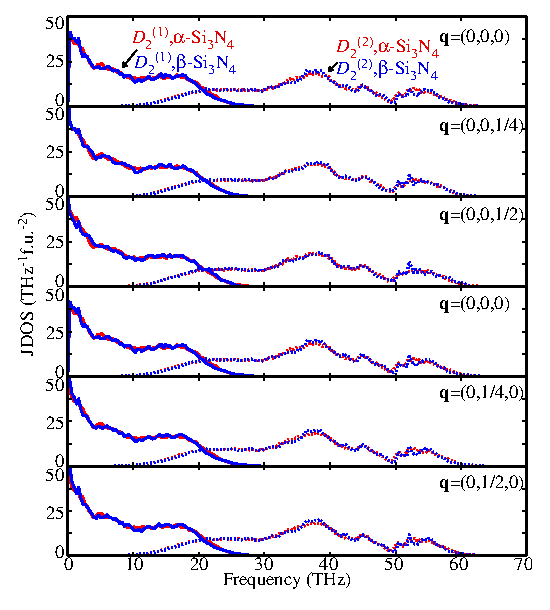
\includegraphics[width=0.9\linewidth]{figure_jdoss.eps} \caption{(color
	  online) \textcolor{blue}{JDOS of $\alpha$- and $\gamma$-Si$_3$N$_4$ at different $\mathbf q$ points.
  The first and and forth rows are JDOS at the same $\Gamma$-point but calculated with the polarization for non-analytic term correction set along $c^*$ and $b^*$, respectively.} \label{fig:Fig6_338} }
 \centering
\end{figure}


In order to analyze the impacts of the selection rules on
the linewidths, we employ the joint density of states (JDOS)
${D_2(\mathbf{q},\omega)}$,
\begin{align}
 \label{eq:jdos}
 &D_2(\mathbf{q},\omega) = D_2^{(1)}(\mathbf{q},\omega) +  D_2^{(2)}(\mathbf{q},\omega)
\end{align}
where 
\begin{eqnarray*}
	D_2^{(1)} & = & \frac{1}{N} \sum_{\lambda'\lambda''}\Delta(-\mathbf{q} + \mathbf{q'} + \mathbf{q''}) \nonumber \\
								   & \times & [\delta(\omega + \omega_{\lambda'} - \omega_{\lambda''}) + \delta(\omega - \omega_{\lambda'} + \omega_{\lambda''})],\\
	D_2^{(2)} & = & \frac{1}{N} \sum_{\lambda'\lambda''}\Delta(-\mathbf{q} + \mathbf{q'} + \mathbf{q''}) \nonumber \\
								   & \times & \delta(\omega - \omega_{\lambda'} - \omega_{\lambda''}),
\end{eqnarray*}
\textcolor{blue}{with $\Delta$($\mathbf{x}$) giving 1 if $\mathbf{x}$ is a reciprocal lattice vector and otherwize zero.}

Fig.~\ref{fig:Fig6_338} shows the frequency-dependences of JDOS at different
$\mathbf{q}$-points on the $\Gamma$--A and $\Gamma$-K paths, which show very slight $\mathbf{q}$-point dependence.
Eq.~(\ref{eq:linewidth}) includes Bose-Einstein functions for the involved
phonon modes and JDOS can be weighted with them as done in
refs.~\onlinecite{mukhopadhyay-ltc,phono3py}, however we omit them for
simplicity. With the weights, the absolute values are affected but the weighted
JDOS of the $\alpha$ and $\beta$ phases are still similar. At the low frequency
region responsible for the LTCs, among the two terms of $D_2^{(1)}$ and
$D_2^{(2)}$ in Eq.~(\ref{eq:jdos}), dominant is $D_2^{(2)}$ which basically
corresponds to the half part ($\omega \geq  0$) of the auto-correlation
function of DOS, which, for the $\alpha$ and $\beta$ phases, commonly show the
frequency gap (Fig.~\ref{fig:Fig5_338_rev}-a).  $D_2^{(2)}$ curves reflect this
DOS feature, dropping suddenly around 0 THz and showing a small shoulder around
5 THz, which corresponds to the width of the gap. Moreover $D_2^{(2)}$ shows a
broad peak around 18 THz, which corresponds to the frequency shift to make the
largest correlation between the higher and lower portions of DOS across the
gap.  Because the gap is basically originated from the differences in the
vibrations of the planer NSi$_3$ commonly contained in the $\alpha$ and $\beta$
phases~\cite{kuwabara}, the major shapes of $D_2^{(2)}$, reflecting this gap
feature, are similar in these phases. With the same origin, the JDOS of
$D_2^{(1)}$ are also similar in these phases. With these similar impacts of
$\Phi_{-\lambda\lambda'\lambda''}$ and JDOS on $\Gamma_\lambda$,
$\Gamma_\lambda$ in Fig.~\ref{fig:Fig5_338_rev}-d are similar.  

As a small but interesting difference in the linewidths between these phases,
$\Gamma_\lambda$ below 5 THz in Fig.~\ref{fig:Fig5_338_rev}-d are aligned on a
smooth line in the $\alpha$ phase, while those in the $\beta$ phase are
scattered roughly onto two different lines. This difference can be explained by
the vibration directions shown in Fig.~\ref{fig:Fig7_338}. In
Fig.~\ref{fig:Fig7_338}-a, $\Gamma_\lambda$ are classified using colors
according to the sums of the squares of the eigenvector components along $\mathbf{q}$; the
sum is 1 for perfectly longitudinal waves. However, these sums have no clear
contrast to distinguish the two branches in the $\beta$ phase.
Fig.~\ref{fig:Fig7_338}-b shows the same plot as Fig.~\ref{fig:Fig7_338}-a, but
with colors according to the sums of the squares of the eigenvector components
along the $a$-$b$ plane, which has 1 when the eigenvectors lie on the $a$-$b$
plane. There is a tendency in the $\beta$ phase that  $\Gamma_\lambda$ are
large for the vibrations along the $a$-$b$ plane. Therefore, within the
single-mode RTA, for the phonon modes below 5 THz, all of which belong to the
acoustic phonon branches, the vibration modes along the $a$-$b$ plane are more
easily scattered in the $\beta$ phase, no matter whether they are longitudinal
or transverse. For the panel of $\beta$-Si$_3$N$_4$ in
Fig.~\ref{fig:Fig7_338}-b, a straight line can divide the phonon modes into the
two groups. The numbers of the phonon modes in the upper and lower parts are
157 and 58, whose ratio is rational as the population ratio of the vibration
modes along and out of the $a$-$b$ plane.


\begin{figure}[ht]
 \centering
  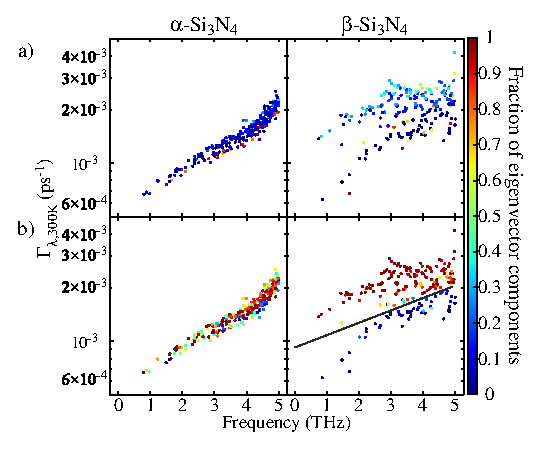
\includegraphics[width=\linewidth]{figure_analyze_gamma3_m1010_print.eps} \caption{(color
	  online) \textcolor{blue}{Distribution of linewidths $\omega_\lambda$ $\leq$ 5 THz
		  with colormaps with respect to strengths of eigenvector compornents along $\mathbf q$ (a)
		  and on $a$-$b$ plane (b).} \label{fig:Fig7_338}} 
 \centering
\end{figure}

% gv weighted dos
%\begin{align}
% \label{eq:v2dos}
% \langle\text{v}^2_i(\omega)\rangle = \frac{1}{N_\mathbf{q}\Omega}
% \int_0^\omega \sum_\lambda
% \text{v}_{\lambda,i}^2\delta(\omega'-\omega)d\omega'.
%\end{align}

\section{Summary}

In the present study, we investigate the lattice thermal conductivities of the
three Si$_3$N$_4$ phases, by using the lattice dynamics based on the {\it
ab-initio} interatomic force constants. The main remarks are as follows:

1) In the $\alpha$- and $\beta$-Si$_3$N$_4$, whose crystal structures are
characterized by the stacking manners of the basal layers, which alter the
LTCs. In $\alpha$-Si$_3$N$_4$, the LTC tensors are rather isotropic, while
$\kappa$$_{zz}$ of the $\beta$ phase is much larger than the others, showing
remarkable anisotropy in the LTC tensor. 

2) In the $\alpha$ phase, the acoustic mode phonons below 6 THz are the main
heat carriers, while in the $\beta$ phase, the phonons below 12 THz contribute
to the thermal conductivity. Their group velocities are significantly different
between the phases; their linewidths are basically similar due to the similar
impacts of the phonon-phonon interaction strengths and selection rules.
Therefore the difference in the group velocities alone qualitatively explains
the difference of anisotropy.

~\textcolor{blue}{3) In the $\gamma$ phase, the frequency distribution of the
phonon mode contributions to LTC is found to be similar to that for
$\kappa$$_{xx}$ of $\beta$-Si$_3$N$_4$ although the respecive phonon properties 
(group velocities and linewidths) are much different from those of the other phases}

\section*{ACKNOWLEDGMENTS}
The present work was partly supported by Grants-in-Aid for Scientific
Research of MEXT, Japan (Grant No. 15K14108 and ESISM (Elements Strategy
Initiative for Structural Materials) of Kyoto University).

\appendix
\section{Pressure dependence of LTC of $\gamma$-phase}
\begin{figure}[ht]
 \begin{center}
  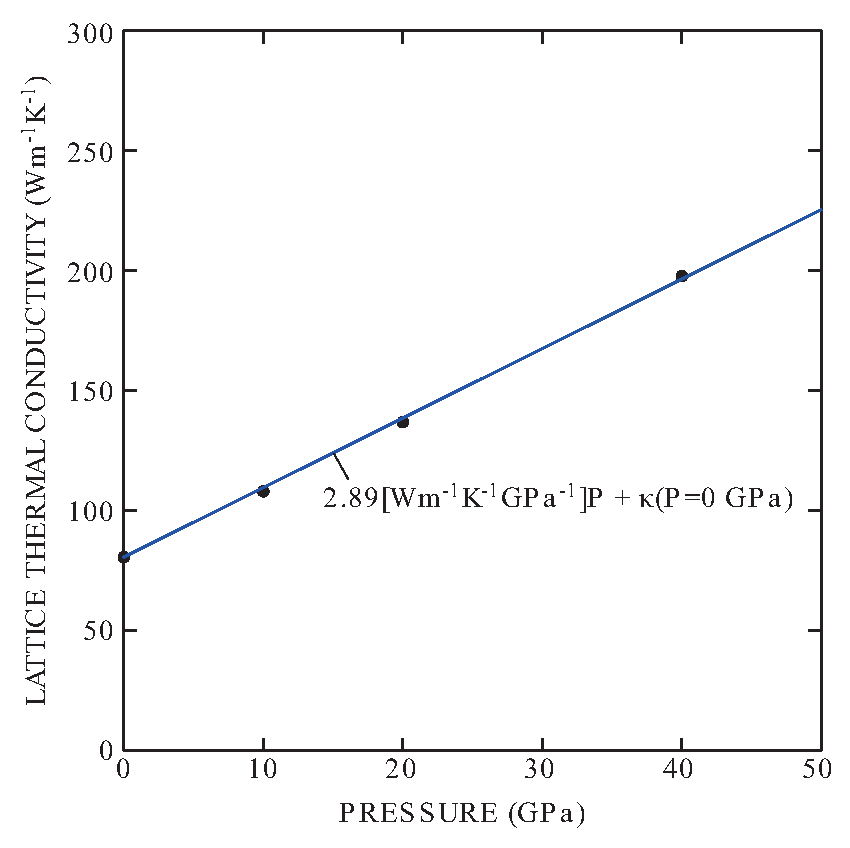
\includegraphics[width=0.80\linewidth]{S1.eps} \caption{(color online)
  Pressure dependence of LTC of $\gamma$-Si$_3$N$_4$.  \label{fig:S1} }
 \end{center}
\end{figure}
\bibliography{Si3N4}
\end{document}
